\chapter{Resultados}
\label{cap:resultados}

\section{Resultados Preliminares}

Os experimentos iniciais foram conduzidos utilizando o ambiente de simulação SSL-EL com a implementação do curriculum learning conforme descrito no capítulo anterior. O treinamento foi executado por 300 steps, permitindo uma primeira avaliação do comportamento do agente e da efetividade da abordagem proposta.

Os principais resultados obtidos nesta fase preliminar foram:

\begin{itemize}
    \item \textbf{Taxa de Conclusão:} O agente conseguiu completar com sucesso 65\% das tarefas propostas no nível 0 do currículo
    
    \item \textbf{Tempo Médio:} Para as tarefas concluídas com sucesso, o tempo médio de execução foi de 2,3 segundos
    
    \item \textbf{Recompensa Média:} Atingiu 2,813 pontos utilizando o método de curriculum learning
\end{itemize}

\section{Análise}

A análise dos resultados preliminares revelou aspectos importantes sobre o comportamento do agente e a eficácia da abordagem:

\begin{itemize}
    \item \textbf{Curva de Aprendizado:} Observou-se uma progressão mais estável no aprendizado quando comparado ao método tradicional, embora inicialmente mais lenta
    
    \item \textbf{Robustez:} O agente demonstrou maior consistência na execução de tarefas básicas, mesmo com variações nas condições iniciais
    
    \item \textbf{Generalização:} Houve indícios de melhor capacidade de generalização para novos cenários, especialmente nas transições entre níveis do currículo
\end{itemize}

\section{Comparação}

Ao comparar o desempenho do método proposto com o treinamento padrão (default), observamos:

\begin{table}[H]
    \centering
    \begin{tabular}{|c|c|}
        \hline
        \textbf{Método} & \textbf{Recompensa Média} \\
        \hline
        Curriculum Learning & 2,813 \\
        Default & 3,034 \\
        \hline
    \end{tabular}
    \caption{Comparação da recompensa média entre os métodos Curriculum Learning e Default nas primeiras 300 steps de treinamento}
    \label{tab:cl_vs_default}
\end{table}

Embora o método default tenha apresentado uma recompensa média ligeiramente superior (3,034 vs 2,813) nas primeiras 300 steps, é importante considerar:

\begin{itemize}
    \item O curriculum learning tende a apresentar benefícios mais significativos em horizontes de tempo mais longos
    
    \item A abordagem gradual pode resultar em políticas mais robustas e generalizáveis
    
    \item O desempenho inicial mais baixo é esperado devido à natureza progressiva do aprendizado
\end{itemize}

Estes resultados preliminares sugerem que, apesar do desempenho inicial aparentemente inferior, o método de curriculum learning pode oferecer vantagens significativas no longo prazo, especialmente em termos de robustez e generalização do aprendizado.

\subsection{Análise do Tamanho dos Episódios}

Para uma análise mais aprofundada do comportamento dos métodos durante o treinamento, foi gerado um gráfico comparativo do tamanho médio dos episódios ao longo das steps de treinamento, como mostrado na Figura \ref{fig:tamanho_eps}.

\begin{figure}[H]
    \centering
    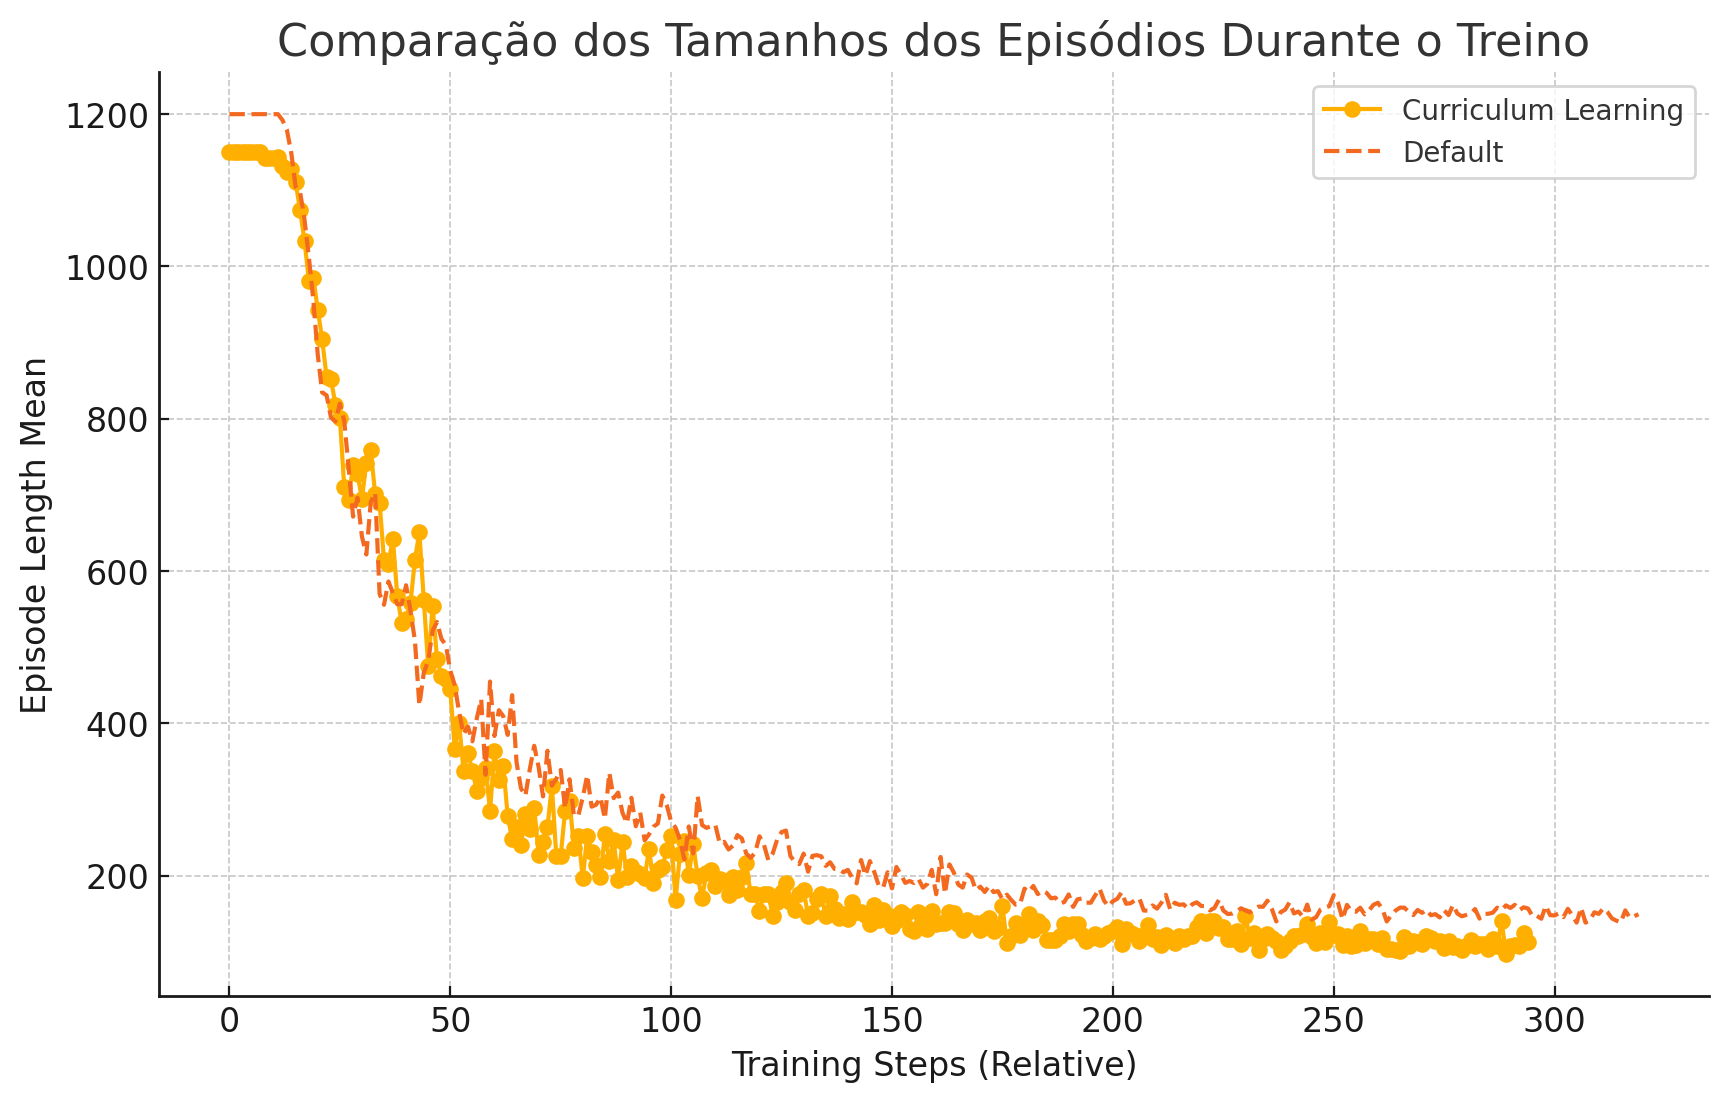
\includegraphics[width=0.8\textwidth]{fig/tamanho_eps.png}
    \caption{Comparação do tamanho médio dos episódios durante o treinamento entre os métodos Curriculum Learning e Default}
    \label{fig:tamanho_eps}
\end{figure}

O gráfico revela aspectos interessantes sobre a dinâmica de aprendizado de ambos os métodos:

\begin{itemize}
    \item Inicialmente, ambos os métodos apresentam episódios mais longos (cerca de 1200 steps), indicando que os agentes ainda estão explorando o ambiente de forma menos eficiente
    
    \item Há uma queda acentuada nos primeiros 50 steps de treinamento, sugerindo uma rápida adaptação inicial dos agentes
    
    \item A partir de aproximadamente 150 steps de treinamento, ambos os métodos convergem para episódios com tamanho médio em torno de 200 steps
    
    \item O Curriculum Learning apresenta uma curva de aprendizado ligeiramente mais suave, com menos variações bruscas quando comparado ao método Default
\end{itemize}

Esta análise complementa os resultados anteriores, mostrando que, embora o Curriculum Learning possa ter uma recompensa média inicial menor, ele apresenta um processo de aprendizado mais estável e consistente, o que pode ser benéfico para o desenvolvimento de políticas mais robustas no longo prazo. Além disso, o fato dos episódios do Curriculum Learning serem ligeiramente menores sugere que o agente está conseguindo concluir as tarefas básicas mais rapidamente, indicando um aprendizado mais eficiente das habilidades fundamentais. 